\chapter{Research methodology}

The aim of this research is to produce a model (and a software that uses it) to infer the emotional state of a player regarding stress and boredom. Since the result of the research is a model, which will be built from different measurements to predict or infer a state, the present work stands on the positivism paradigm. Essentially this work will formulate a theory about how the variation of physiological signals relate to stress/boredom levels in the context of games and how it can be remotely detected. The involvement of humans in the process might relate to the social side of interpretivism, however the foundation of the work is still based on the analysis of physiological signals. Such signals and their patterns might be different for each person, however they are still ordered and regular under the human being perspective. As a consequence, they can be objectively observed, measured and analysed with a quantitative approach and hypothesis testing.

The strategy used to build and validate the knowledge in this project is experimental research. Such approach is composed of a set of research designs that use controlled testing and manipulation of variables in order to understand casual processes. The foundation of an experiment is to manipulate a variable (or a set of them) and measure any changes in other variables. It establishes the effect on a dependent variable, which is the focus of the research. The model being constructed in this research links the variations of physiological signals to stress/boredom levels in the context of games, hence there is a causal effect in the process since identified variations (cause) will precede changes in stress/boredom levels (effect). It progresses to the construction of a hypothesis where the cause will consistently lead to the same effect so the link between variations of signals and emotional levels can be inferred or predicted.

\section{Research objectives}

This research is expected to produce a method that is able to interpret remotely acquired signals from a person and detect his/her current emotional state regarding stress and boredom according to data obtained in a calibration phase. The model will be implemented in a software that uses a video feed to detect the person's emotional state.

The following research objectives (O) have being identified to support the overall aim of this thesis:

\textbf{O1}: identify the main concepts, theories and signals associated with the psychophysiological profile of users and their emotions within the field of HCI, particularly regarding games research. The result of this objective is a formal definition of stress and boredom within the context of this research, as well as the identification of which physiological and non-physiological signals are commonly applied to emotion detection.

\textbf{O2}: identify the ideal existing computer vision techniques that can be employed to remotely extract the identified physiological and non-physiological signals of users via analysis of videos. The investigation includes the analysis of how existing techniques are being applied to emotion detection. The set of signals to be remotely extracted is based on the results of objective \textbf{O1}.

\textbf{O3}: investigate the feasibility, accuracy and challenges of applying the identified computer vision techniques regarding the extraction of the signals within the context of computer games. This objective also comprehends the analysis of the behavior of players during gaming sessions and how it affects the technique.

\textbf{O4}: investigate and validate the concept of a game-based calibration phase as an emotional elicitation source able to provide data to fit a user-tailored predictive model. The result of this objective is to design and validate a set of calibration games that can trigger the emotional responses required for the analysis of the remotely obtained signals and detection of boredom/stress levels by the model.

\textbf{O5}: Propose and validate a user-tailored, multifactorial model that uses the identified physiological and non-physiological signals, the computer vision technique and the calibration data to detect the current stress/boredom levels of a person while he/she plays any video game.

%The objective of this research is to produce a method that is able to interpret remotely acquired signals from a person playing a game and detect his/her current emotional state regarding stress and boredom according to data previously obtained in a calibration phase. The model will be implemented in a software that uses a video feed to detect the person's emotional state.

%The current approaches used to obtain information from the players during games research inevitably affect the player's experience. They require the user to stop the game activity in order to share his/her current state, such as by answering a questionnaire. The frequency that such questionnaires are issued is also a concern. If performed too often, more information might be collected, but the data might contain noise caused by the frequent interruptions, e.g. player is more stressed/bored by the questionnaire interruptions than by the game itself. If performed too sparse, not enough information will be gathered from the player. A physical sensor attached to a player, on the contrary, allows a continuous monitoring process, however it is intrusive and might interfere with the player capacity to interact with the game. It might prevent the use or movement of specific parts of the body, for instance. Physical sensors also increase the chances of the player to behave differently as a side-effect of the monitoring process itself.

%A purely remote-based solution, as the one proposed by this research, enhances the tooling available to the games research community regarding investigation methods of stress and boredom. A games researcher will be able to increase the internal validity of his/her workflow by ensuring the player keeps the focus on the game without interruptions and by minimizing the side effects (and inconveniences) of physical monitoring. This research could also be deployed as a solution for game developer studios to automatically analyze hours of recorded gameplay and highlight the moments when boredom/stress levels changed significantly. As a complement the solution will be based on a single, ordinary camera and a software implementation, which eliminates the use of complex setups of physical sensors. It eases the investigation process and reduces costs.

\section{Research process}
\label{sec:research-process}

The research will initially proceed from a systematic literature review regarding emotions and their detection/identification. The scope of the survey will be narrowed to the field of HCI and games research. Searches in complementary fields might happen when key concepts that were identified require additional definition. This initial literature review will fulfill objective \textbf{O1}, producing the identification of which physiological and non-physiological signals and approaches are applied to the problem of emotion detection.

A second systematic literature review will follow focusing on the identification of which computer vision techniques can be employed to remotely extract the signals identified in the first literature review. The scope of the survey will be the field of computer vision and HCI. The selection criteria for the techniques will be capabilities regarding remote acquisition of information and applicability within the fields of HCI and/or games research. The accuracy and performance of each techniquine will be analyzed and compared based on published materials. The result of the second literature review will be the selection of the most efficient computer vision techniques that can be used to remotely extract the user signals idenfitied in the first literature review. It will fulfill objective \textbf{O2}.

After the definition of which user signals and computer vision techniques will be employted for emotion detection, a series of experiments will be conducted. The first experiment will focus on collecting data to fulfill objectives \textbf{O3} and \textbf{O4}. The experiment will be designed around the use of games for emotion elicitation, which will produce data regarding variations of physiological and non-physiological signals and their relation to emotions. The resulting data will be analyzed to test the hypothesis that games can be used as elements of emotion elicitation within the context of this research, which accounts for objective \textbf{O4}. Further tests will be performed involving the computer vision techniques and the ground truth signals measured during the experiment. Those tests will check the feasibility and accuracy of the computer vision techniques within the context of games, in particular the context of this research. Results regarding this analysis will fulfill objective \textbf{O3}.

Based on the data collected during the first experiment, a user-tailored model will be developed. A sequence of experiments will be designed and conducted to refine and validate the capacity of the proposed model to detect emotional states as stress and boredom. The cycle of experimental validation and model refinement will end when the model is proved to accurately detect the emotional state of players, which fulfills objective \textbf{O5}.

%The experiment design will be based on a within-subject approach \cite{lane2015online}. In such approach, all participants perform at all levels of the treatment and there are no control groups. It is the opposite of a between-subjects approach, where subjects are divided in more than one group that receive different treatments. In that approach there are special groups, called control groups, that receive no treatment. The comparison between the control groups and the treatment groups ensures internal validity. In the context of this research, physiological signals will be measured, so the division of subjects into more than one group poses a comparison problem. Each individual will inevitably differ from one another regarding physiological signals, such as variations in average HR during rest, for instance. When measuring HR, for instance, some subjects will have higher/lower HR mean than others, independent of the group they are in or the treatment they undergo. To counter that problem, the experiment will use a one-group posttest design \cite{kirk1982experimental}, as illustrated by Figure \ref{fig:experiment}. Using the first row as an example, subject $S_0$ played game $G_a$ as the first level of the treatment, followed by a post-test of that game ($PT_a$), then a rest period. In the second level of the treatment, the subject played game $G_b$, followed by a post-test of that game ($PT_b$), then another rest period. Finally in the third level of the treatment, the subject played game $G_c$ followed by a post-test of that game ($PT_c$).

%\begin{figure}[ht]
%    \centering
%    \includegraphics[scale=0.5]{imgs/experiment-design.png}
%    \caption{One-group posttest experiment design used in this research. $S_j$ represents the $j^{\text{th}}$ subject, $G_i$ represents a game of type $i$, $PT_i$ is the post-test for game $G_i$ and $rest$ is a resting period.}
%    \label{fig:experiment}
%\end{figure}

%By using a one-group posttest design, each individual will perform on all levels of the treatment (play a set of different games). The within-subjects approach ensures that the differences between subjects are not interfering in the comparison, since a subject is being compared to his/herself in the different levels of the treatment. Subjects are not being compared among each other. In essence, each subject is serving as his/her own control group. According to Kirk \cite{kirk1982experimental}, the one-group posttest design should only be used when the researcher knows the mean value of the independent variable when no treatment is in effect. Such information will be obtained during the resting periods of the experiment, where the baseline value for all measured signals can be established for each subject.

%The process of sampling a group of participants for each experiment will follow the convenience sampling approach, a non-probability sampling technique where participants are recruited because of their convenient accessibility/proximity to the researcher. Volunteers will be randomly recruited for each experiment. A probability sampling approach, where each individual of the population has an equal chance of being selected, would be ideal and would strength the external validity of the research. However the costs, logistics and time constraints associated with it makes such approach impractical in the context of this research.

\section{Current state of research}

The current state of this research is illustrated in Figure \ref{fig:research-current-state}. Both objectives \textbf{O1} and \textbf{O2} have already been fulfilled. After the first literature review, the accomplishment of \textbf{O1} produced the identification of the main concepts, theories and signals associated with phychophysiological profile of users and their emotions. Chapters \ref{ch:literature-games}, \ref{ch:literature-physiological} and \ref{ch:literature-multifactorial} present the results of such literature review. The results of the literature review regarding objective \textbf{O2}, which focus on the identification of ideal existing computer vision techniques to remotely extract signals from users, is presented in chapters \ref{ch:literature-face} and \ref{ch:literature-face}. The investigation also produced a publication regarding emotion detection and remote measurement of physiological signals \parencite{bevilacqua2015proposal}.

\begin{figure}[ht]
    \centering
    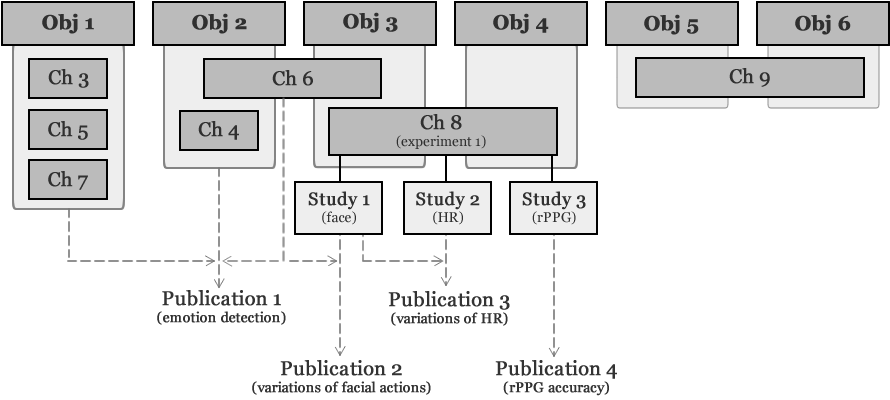
\includegraphics[width=0.8\textwidth]{figures/research-current-state.png}
    \caption{Current state of this research.}
    \label{fig:research-current-state}
\end{figure}

Objective \textbf{O3} is being finalized. The aim of that objective, which is the investigation of feasibility, accuracy and challenges regarding the application the computer vision techniques within the context of games, was performed as an experiment. The experiment and the three studies conducted on the collected data are described and presented in chapter \ref{ch:experiment1}. Each one of those studies resulted in a publication, which present results regarding variations of facial actions \parencite{bevilacqua2016variations}, variations of heart rate \parencite{bevilacqua2017changes} and accuracy evaluation of the selected computer vision technique \parencite{bevilacqua2017accuracy}. The last two aforementioned publications were recently submitted for review. The main challenges regarding the application of the computer vision techniques within the context of games have already been identified. A publication \parencite{bevilacqua2017accuracy} and the literature review presented in chapter \ref{ch:literature-face} show the limitations of the computer vision technique when applied to contexts of games research involving natural behavior of users, e.g. head movement and face oclusion. A new study will be conducted to investigate ways to improve the computer vision technique to eliminate or mitigate such limitations.

Objective \textbf{O4} has been partially fulfilled. A pilot study, an experiment (described in chapter \ref{ch:experiment1}) and two publications \parencite{bevilacqua2016variations,bevilacqua2017changes} describe and validate the concept of calibration games. Up to the present moment, however, the variation of the signals produced by such calibration games have not been employed in any studies or experiments involving emotion detection, so its utility within the context of this research needs to be further investigated.

For information regarding future work, refer to chapter \ref{ch:closing}.
